\documentclass{article} % For LaTeX2e
\usepackage{graphicx}
\graphicspath{ {images/} }
\usepackage{nips14submit_e,times}
\usepackage{hyperref}
\usepackage{cleveref}
\usepackage{subcaption}
\usepackage{url}
%\documentstyle[nips14submit_09,times,art10]{article} % For LaTeX 2.09

\title{Automatic Target Detection and Classification: \\
  Deep Learning on Low Power Platforms}

\author{
  Asst. Prof. Mark Silberstein \\
  mark@campus.technion.ac.il\\
}

\newcommand{\fix}{\marginpar{FIX}}
\newcommand{\new}{\marginpar{NEW}}

\nipsfinalcopy % Uncomment for camera-ready version

\newcommand{\cropsrow}[3]{\includegraphics[width=0.15\textwidth]{images/crops/#1.jpg} & #2 & \includegraphics[width=0.15\textwidth]{images/crops/mask_#1.jpg} & #3}

\begin{document}

\maketitle

\section{Summary}

Over the last decades the use of Unmanned System has proven very beneficial in
saving life of military personal and cutting the costs of operational tasks.
Still, these systems require a `Man in the loop'. This requirement increases the price
of these systems and limits their availability.
The recent years have seen a leap in machine learning algorithms and available
computing power. These advances enable computers accomplish tasks
previously considered possible only by humans.
This opens the path to Unmanned Autonomous Systems (UAS).
Many times the UAS are limited by size. On the other hand, the state of the
art machine learning algorithms require high computing power. These two
constraints collide with each other.
The new generation of low power high performance platforms like the NVIDIA
Jetson TX1, opens the path to new applications for size limited UAS.
In this research we harness the power of these platforms to develop machine vision
algorithms for UAS using state of the art Deep Learning techniques. 

This research is performed in cooperation with the Technion AUVSI project team.
This project is a collaboration between the Aerospace and Electrical engineering
faculties, in which students design and build Unmanned Autonomous aerial system
to compete in the AUVSI students competition.

\section{Background}

\subsection{Deep Learning}
\label{sec:classical_mv_solution}

Classical machine learning, traditionally approaches classification problems
by first transforming the data from the problem space to some feature
space. The data in this feature space is hopefully invariant to transforms common
in the problem space, e.g. similarity and affine transforms, occlusion, lighting
etc. It is assumed that in this feature space, objects of the same class reside
in some manifold and the manifolds of different objects are separated by regions
of low density. A classifier, e.g. SVM is trained on this feature space to
discriminate between object of different classes.

This approach has been applied successfully to problems in many fields. But
finding the right
feature space for the problem and the right classifier for the feature space is
a complicated task that requires expertise.

During the last years, Deep Learning (DL) proves to be the De-facto method for
many artificial intelligence tasks. One of the main advantages of DL is that
it automatically learns the feature space. Thus the feature space is custom
tailored for the specific problem.


\subsection{AUVSI project}

The Association for Unmanned Vehicle Systems International (AUVSI)
organizes the Student Unmanned Aerial System (SUAS) competition
\url{http://www.auvsi-seafarer.org/}. The competition is aimed  at
stimulating and fostering interest in unmanned system technologies.
The  student  are required  to  develop  and  provide  the  analysis,
design, fabrication and demonstration of a system capable of completing
specific autonomous aerial missions.

One of the missions is the automatic detection and classification of targets.
Some targets are characterized by different geometric shapes and color. Another
target, in the form of a QR code requires high spatial resolution. Another
target is a doll in the form and size of a human. This target simulates
a search and rescue operation.~\cref{fig:targets} shows
some of the targets used in last year's competition.
\begin{figure}[h]
	\centering
	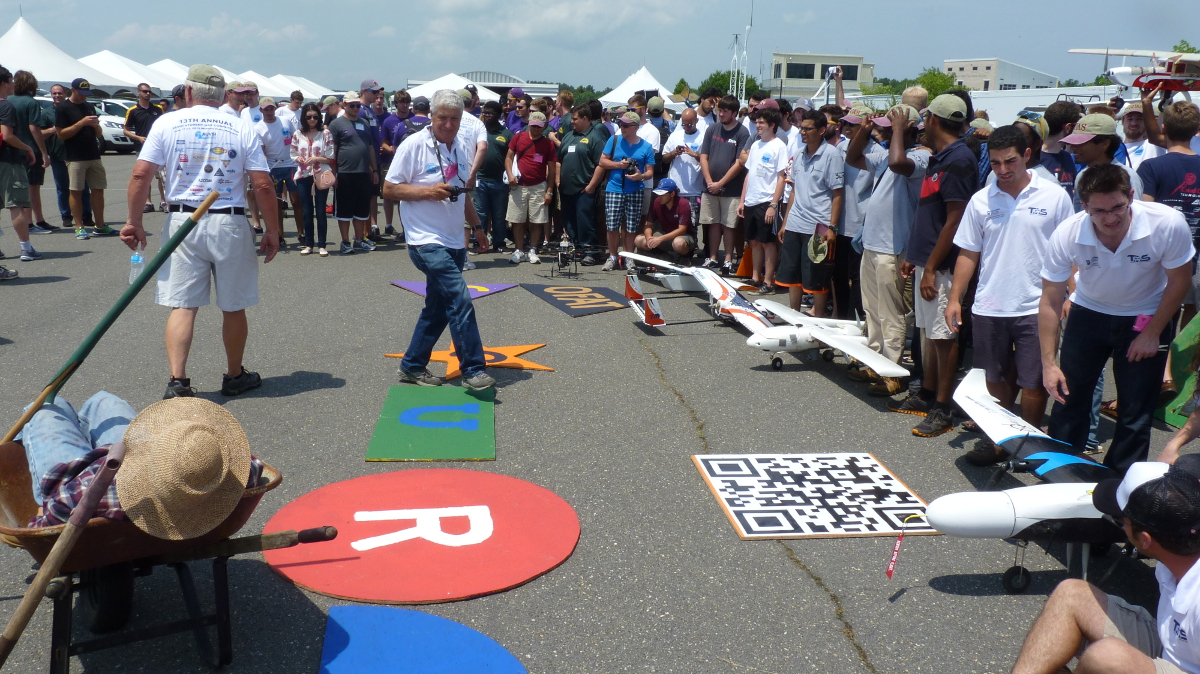
\includegraphics[width=0.8\textwidth]{auvsi_targets}
	\caption{Example of targets used in the 2015 AUVSI competition.}
	\label{fig:targets}
\end{figure}

This is the third year that the Technion participates in the AUVSI SUAS
competition. Last year the Technion team achieved 2\textsuperscript{nd} place
among more than 30 teams from universities all around the world.

\section{Proposed Research}

\subsection{Target Detection and Classification}

The task of target detection and classification is related
to surveillance, `search and rescue', `friend or foe' identification and many other security related missions. 
The Region Convolutional Neural Networks
(R-CNN)~\cite{Girshick2014} revolutionized the area of object detection, classification, and segmentation. Fig.~\ref{fig:RCNN} show the diagram of a typical
R-CNN system. It is made of two stages, the first is a region proposal stage that extracts
object candidates. This regions are stretched into a predefined patch size and then
fed into a CNN. The CNN calculates confidence levels for a set of objects it was trained
for.
\begin{figure}[h]
	\centering
	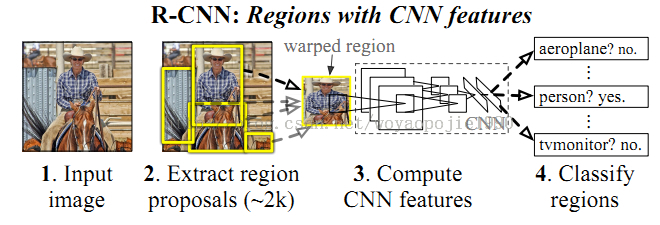
\includegraphics[width=0.8\textwidth]{RCNN}
	\caption{Diagram of a RCNN system}
	\label{fig:RCNN}
\end{figure}

We implemented a system based on R-CNN architecture to detect and classify the
targets in the AUVSI competition. The system is comprised of two subsystems shown in \cref{fig:shape_diagram,fig:letter_diagram}.
The first subsystem detects and classifies target shapes in full (downscaled) image. The
input to this subsystem is a down-sampled version of the original image. The output is square crops classified as one of the possible target shapes (circle, half circle, cross, rectangle, etc.). Crops are taken from the full resolution
image and are fed into the
next subsystem that classifies the characters inside the shape. These subsystems
thus work as a cascade of classifiers. This hierarchical coarse to fine setup enables good classification performance using smaller DL networks.
\begin{figure}[h]
	\centering
	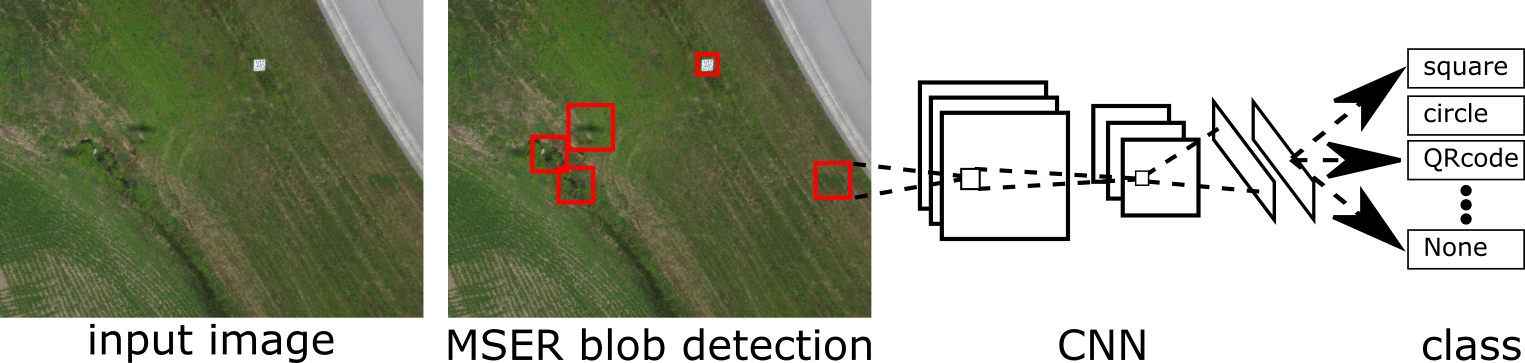
\includegraphics[width=0.8\textwidth]{diagram}
	\caption{Diagram of the shape classification subsystem}
	\label{fig:shape_diagram}
\end{figure}
\begin{figure}[h]
	\centering
	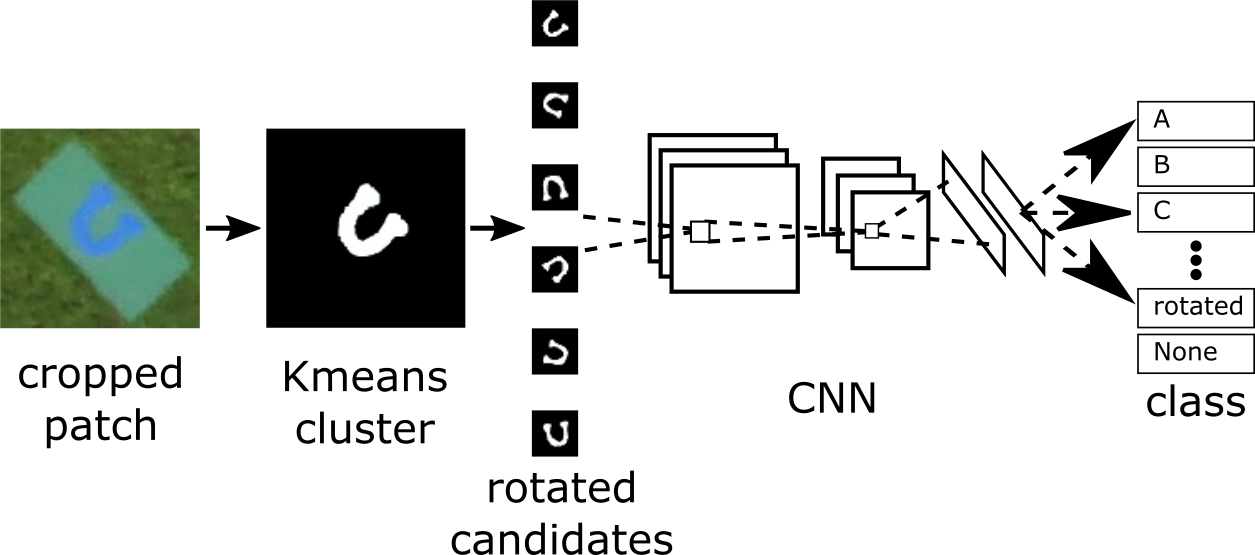
\includegraphics[width=0.5\textwidth]{letter_diagram}
	\caption{Diagram of the character classification subsystem}
	\label{fig:letter_diagram}
\end{figure}

\subsection{Low Power Computing}

% Short description of the Jetson TX1
% Results of Ahmad
The Jetson TK1,~\cref{fig:jetson}, offers both a general purpose CPU and a powerful GPU
in a low power, small form factor plaform. The GPU enables fast calculation of DL networks.
Using the Jetson TK1 and the Caffe~\cite{jia2014caffe} DL network, we
are developin a low power, real-time target detection and classification system.
The later enables fast calculation of the DL network.  
\begin{figure}[h]
	\centering
	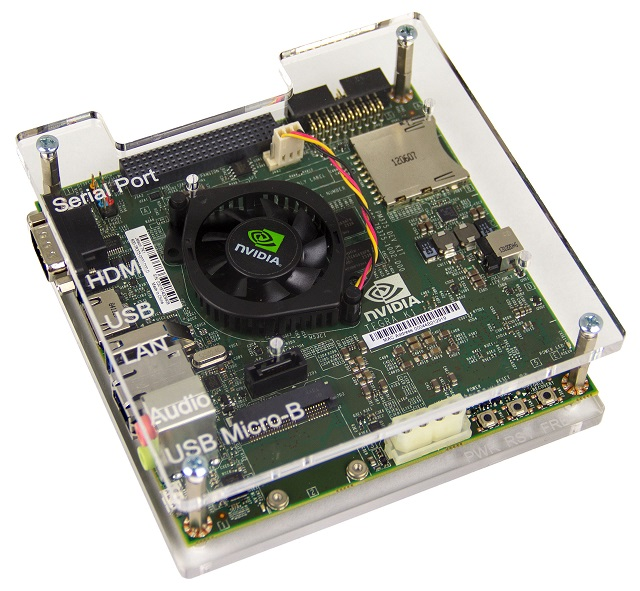
\includegraphics[width=0.8\textwidth]{jetson}
	\caption{The Jetson TK1 by NVIDIA}
	\label{fig:jetson}
\end{figure}

Initial results show that 

\begin{center}
	\begin{tabular}{ | l | l | }
		\hline
		Stage 										& Time [ms] 	\\ \hline
		Target Detection (CPU) 						& 200      		\\ \hline
		Low Resolution Classification (GPU) 		& 10 			\\ \hline
		High Resolution Classification (GPU)		& 10 			\\ \hline
		Total 						 				& 220 			\\ \hline
	\end{tabular}
\end{center}

\subsection{Demonstration system}

% Description of the Ground System
% Details of Next year Gannt.

\subsection{Shape Classification}
\label{sec:shape_class}

The first stage of shape classification is region proposal. I used the MSER feature
descriptor as blob detection. MSER detects regions (in gray scale images) that are
stable when different binarization threshold are applied to the image. In other
words MSER detects simply connected regions that look `differently' from their
surrounding (either darker or brighter). I always select a square patch centered
around the blob. This is in contrast to R-CNN where there region is selected as is
and then stretched into a square patch. The reason is that I don't want the geometric
shapes to be distorted, e.g. a circle to turn into an ellipse, a square into a rectangle
etc.

I decided to start with the CIFAR-10 CNN included in the Caffe. And in the end the
only change I did was to add a dropout layer before the fully connected layer 
(see \cref{fig:full_net}).
\begin{figure}[h]
	\centering
	\includegraphics[width=\textwidth]{full_net}
	\caption{Diagram of the shape classification Caffe network}
	\label{fig:full_net}
\end{figure}
The motivation for using the CIFAR-10 network was that I had $\approx10$ geometric
shapes to classify and the basic network achieved high accuracy in training ($>99\%$).
The classes I trained the net to classify are: `circle', `half circle', `rectangle',
`triangle', `cross', `pentagon', `hexagon', `star', `qrcode', `no target'. Note the
last class, `no target'. It is needed as the region proposal algorithm has a very high
false positive rate (i.e. returns many patches with no target inside~\cref{fig:multiple_region_suggestions2})
\begin{figure}[h]
	\centering
	\includegraphics[width=0.8\textwidth]{multiple_region_suggestions2}
	\caption{Example of regions selected by the MSER algorithm}
	\label{fig:multiple_region_suggestions2}
\end{figure}
I trained the network on synthetic samples (see~\cref{fig:image_with_targets} and~\cref{sec:data_synthesis}) using three
constant learning rates (same as in the Caffe tutorial). The largest training set comprised of
$500K$ samples, half of them with target of random shape, color, character, orientation and scale.
The other half are patches with no target with them.
\begin{figure}[h]
	\centering
	\includegraphics[width=0.8\textwidth]{image_with_targets}
	\caption{Synthetic targets (the only true target is the star at the top right with character `C')}
	\label{fig:image_with_targets}
\end{figure}

The network is trained for $\approx150$ epochs. Before adding the dropout layer the
network achieved $>99\%$ accuracy. I added a dropout layer before the fully connected layer to
avoid over-fitting.

Patches classified as `no-target' are dismissed. The rest of the patches are re-cropped from
the full resolution image and passed on to the character classification subsystem.

\subsection{Character Classification}
\label{sec:char_class}

The purpose of the character classification subsystem (\cref{fig:letter_diagram})  is to classify
the character inside the targets and its orientation. Its input are patches (taken from
the full resolution image) that were classified as containing target shapes. The first stage is
segmentation of the pixels belonging to the character. This is done using the `k-means' clustering
algorithm in the following manner:
\begin{enumerate}
	\item All the pixels in the patch are clustered according to their color into to groups: shape
	and background. The assumptions that allow this is that the background in the patch is relatively
	uniform. And that the number of pixels belonging to the character are relatively small.
	\item The pixels belonging to the cluster closer to the patch center are assumed to be the
	shape. A binary `shape' mask is formed by selecting these pixels.
	\item Any holes in the `shape' mask are filled (this is done in case the character pixels are
	colored clustered with the pixels belonging to the background).
	\item Pixels marked by the mask are clustered again by their color. The pixels belonging to tohe
	cluster closer to the patch center are assumed to belong to the character.
	\item A binary `character' mask is formed by selecting these pixels. See \cref{tab:patches} for 
	example of patches and their corresponding `character' mask.
\end{enumerate}

The `character' mask is rotated at a angles $0^\circ,15^\circ,30^\circ,\dots,345^\circ$ and re-cropped
tightly. This procedure forms $12$ copies of the binary mask at different angles (see \cref{fig:letter_diagram}).
These masks are re-sampled at $28\times28$px resolution and fed into a CNN trained for classifying
characters.

The CNN (\cref{fig:alpha_NN}) is based on the MNIST Caffe example, with a dropout layer.
\begin{figure}[h]
	\centering
	\includegraphics[width=\textwidth]{alpha_train_test}
	\caption{Diagram of the character classification Caffe network}
	\label{fig:alpha_NN}
\end{figure}
It is trained to classify the input gray-scale patch into one of 28 classes: 26 uppercase characters,
`rotated' class, and `None' class. I added the `rotated' class because without it the
network would have a very high rate of false positives on rotated patches (i.e. it
would classify rotated characters wrongly as another character). The output of the network
is the probability score that the patch belongs to one of the 28 classes. If the class
with the highest probability is either `None' or `rotated', or that the probability of
the class is lower than some threshold, then the patch is dismissed as `no-target'.
I set the threshold empirically to 0.95.

As mentioned before the network is fed with 12 copies of the `character' mask rotated at
different angles. For each angle the network either discards the patch or selects for it
some character class.
The angle, whose character class receives the higest probability, is selected as the shape
orientation and the corresponding class is used as the shape character. If all the rotated
patches are discarded by the network, then the patch itself is discarded as `no-target'.
This way the character classification subsystem is used also as a weak target classifier. 

The network was trained with data from the following groups:
\begin{itemize}
	\item Straight (not rotated) characters. The character were drawn using random
	font, $\pm10^\circ$ orientation, scale and translation.
	\item Rotated characters. The same as above but the character was randomly rotated
	at the range $15^\circ$ to $345^\circ$.
	\item None. This class represents empty patches wrongly classified by the
	shape classification algorithm as targets. It is created by randomly cropping background
	patches and passing these through the `k-means' clustering algorithm described above.
\end{itemize}
The data comprised of $300$K samples equally divided between the above groups.

\section{Data Synthesis}
\label{sec:data_synthesis}

By far, the largest increases in the system performance were achieved by improving
the data synthesis process. The improvements involved understanding the type of
patches that the network `sees' in practice. Before this, the system would have
a very high rate of false positives (empty patches classified as valid shapes) and
false negatives (real targets classified as `no-target'). The first problem was
solved when I noticed that the region proposal algorithm select patches at 
multiple sizes, while the 'no-target' patches I synthesized where always of the
same size. Synthesizing patches of different sizes~\cref{fig:random_no_target}, drastically
reduced the rate of false positives.
\begin{figure}[h]
	\centering
	\includegraphics[width=0.3\textwidth]{data_synthesis3}
	\caption{Example of random scale `no-target' patches.}
	\label{fig:random_no_target}
\end{figure}

The problem of false negatives was caused by the fact that the region proposal
algorithm does not crop `tightly' around the target shape~\cref{fig:sub1} while
the synthesized targets were drawn at the center of the patch~\cref{fig:sub2}
and tightly cropped. Loosening the `tight' cropping of the synthetic examples~\cref{fig:sub3}
decreased the number of false negative classifications.
Loosely placing 
\begin{figure}[h]
	\centering
	\begin{subfigure}{.3\textwidth}
		\centering
		\includegraphics[width=.3\linewidth]{R}
		\caption{Proposed target region}
		\label{fig:sub1}
	\end{subfigure}%
	\begin{subfigure}{.3\textwidth}
		\centering
		\includegraphics[width=.3\linewidth]{data_synthesis1}
		\caption{Tightly cropped sample}
		\label{fig:sub2}
	\end{subfigure}
	\begin{subfigure}{.3\textwidth}
		\centering
		\includegraphics[width=.3\linewidth]{data_synthesis2}
		\caption{Loosely cropped sample}
		\label{fig:sub3}
	\end{subfigure}
	\caption{Imitating the way the region proposal algorithm crops around targets.}
	\label{fig:data_synthesis}
\end{figure}

The background of all synthetic data (targets and no-targets) were randomly cropped
from a subset of the $\approx1000$ images taken during the competition flight.
The background images were selected so that they will not include targets (that
might accidentally appear in `no-target' patches) on the one hand, and will include
as much clutter as possible (people, cars etc.), on the other hand.
It is important that the system used in next year's competition will be trained with
background images taken at multiple scenarios (different weather, time of day etc.). 

\section{Implementation}

The project was implemented using the Caffe~\cite{jia2014caffe} DL framework.
The Caffe framework was used through the python interface. This allowed for 
fast prototyping. Another benefit of using the Python interface was that I
was able to freely use it on the on EC2 amazon servers where I trained the Caffe
models.

The EC2 servers I used have a GRID K520 GPU. Training of a typical network ranges
from 2 to 6 hours depending on the data size. Classification of single image
takes approximately 600ms.

\section{Results}
\label{sec:results}

The system was validated on $\approx400$ images taken during the target detection mission
of the competition (the rest of the $>600$ images not used for validation were taken
during other missions). The small number of targets that appear in this images (four shape
and one QR targets) means that the validation is only qualitative and doesn't have
real quantitative value. Nonetheless this is the best I could do to imitate a real
competition scenario, and serves for comparing different networks performance.

In the following figures, regions classified as non-target by the shape classifier are
marked by red square. Regions classified as valid shapes by the shape classifier but
as no-target by the character classifier are marked by yellow square. Regions classified
correctly by both subsystems are marked by blue square. \Cref{fig:true_positive1,fig:true_positive2} show two examples of targets classified
correctly both by the shape subsystem and the letter subsystem. 
\Cref{fig:false_positive1,fig:false_positive2} show two examples of non-target regions
(marked by yellow square) misclassified by the shape classifier but correctly classified
by the character classifier (the region classified as `qrcode' in~\cref{fig:false_positive2}
is an exception as it doesn't include a character and therefore its character classification
as no-target is invalid). \Cref{fig:misclass} is an example a target classified as the wrong
shape (triangle instead of half-circle). This is the only shape misclassification in the
validation set. \Cref{fig:false_negative1} is an example of a target misclassified as no-target
by the shape classifier. This is the only target in the validation set that the system missed.

\Cref{tab:patches} shows examples of pathces classified as shapes (both true and false positives),
their `character' mask, and character classification.
\begin{figure}[h]
	\centering
	\includegraphics[width=0.8\textwidth]{true_positive_correct_letter1}
	\caption{Target classified correctly as: shape=rectangle, char=U and angle=$30^\circ$.}
	\label{fig:true_positive1}
\end{figure}
\begin{figure}[h]
	\centering
	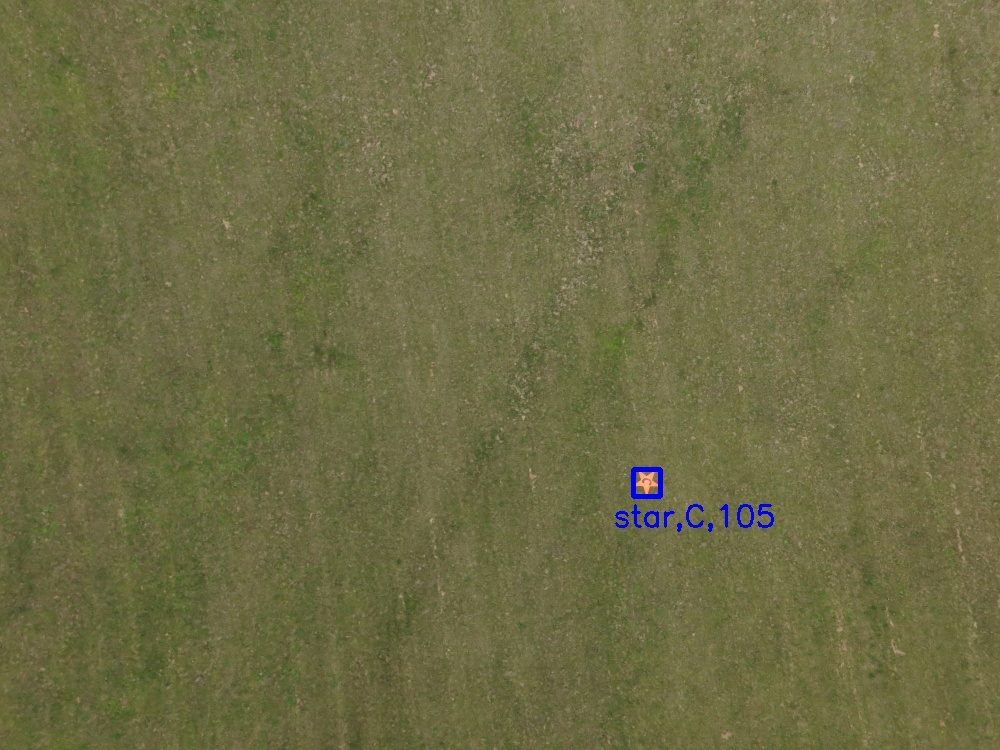
\includegraphics[width=0.8\textwidth]{true_positive_correct_letter2}
	\caption{Target classified correctly as: shape=star, char=C and angle=$105^\circ$.}
	\label{fig:true_positive2}
\end{figure}
\begin{figure}[h]
	\centering
	\includegraphics[width=0.8\textwidth]{false_postive_weak_classification1}
	\caption{Example of false positive of the shape classification but correct character classification.}
	\label{fig:false_positive1}
\end{figure}
\begin{figure}[h]
	\centering
	\includegraphics[width=0.8\textwidth]{false_postive_weak_classification2}
	\caption{Example of false positive of the shape classification but correct character classification.}
	\label{fig:false_positive2}
\end{figure}
\begin{figure}[h]
	\centering
	\includegraphics[width=0.8\textwidth]{misclassfication}
	\caption{Shape misclassification: Half circle target misclassified as triangle.}
	\label{fig:misclass}
\end{figure}
\begin{figure}[h]
	\centering
	\includegraphics[width=0.8\textwidth]{false_negative1}
	\caption{False negative: the shape classifier misclassified the star target as `no-target'.}
	\label{fig:false_negative1}
\end{figure}

In an effort to improve performance I tried to replace the single shape network by
an ensemble of networks.
I trained three shape networks (of the same model) on three different sets of data. Each
one of the data sets included $150$K samples. But in the validation the use of an ensemble of
networks increased the number of false negatives (missed targets). Nonetheless I think that
ensemble of networks is a worthwhile direction and increasing the number of networks
might improve its performance.

\begin{table}[ht]
\centering
\begin{tabular}{llll}
\multicolumn{1}{c}{\bf crop}  & \multicolumn{1}{c}{\bf shape class.} &\multicolumn{1}{c}{\bf `character' mask} &\multicolumn{1}{c}{\bf letter class.} \\
\hline
\cropsrow{1}{`CROSS'}{NO TARGET} \\
\hline
\cropsrow{2}{`RECTANGLE'}{`U' at $30^{\circ}$} \\
\hline
\cropsrow{5}{`CIRCLE'}{`R' at $315^{\circ}$} \\
\hline
\cropsrow{7}{`QR code'}{no target} \\
\hline
\cropsrow{16}{'QR code'}{no target} \\
\hline
\cropsrow{17}{CROSS}{no target} \\
\hline
\cropsrow{27}{`STAR'}{`C' at $105^{\circ}$} \\
\hline
\end{tabular}
\caption{Crops classified as valid targets and their Alphanumeric classification.}
\label{tab:patches}
\end{table}

\section{Conclusions and Future Work}

This project demonstrates the capability of deep-learning networks to solve
`real world' problems. It also shows that it is possible to train a network on synthetic
data. But it is important that the data will fit the classification process.

We are already in the process of recruiting the students for next year's
competition. The results of this project offer a starting point
for exploring new ideas:
\begin{itemize}
\item Try ensemble of small DL networks.
\item Explore other network architectures.
\item Explore other region proposal algorithms (e.g. based on color statistics).
\item Train the network on different scenarios (different wheather, time of day etc.).
\end{itemize}

Recently NVIDIA released mini boards with strong GPU's \url{https://developer.nvidia.com/jetson-tk1}. It can be interesting to try
to implement a similar system on a board like this. This board can serve as the computer
on-board the drone. Thus the image processing tasks can be performed `in the air' and not in the ground station as it is done today.

\section{Budget Plan}

\begin{center}
	\begin{tabular}{ | l | l | l | }
		\hline
				& Item 											& Budget (NIS) 	\\ \hline
		1		& MSc Student 									& 20,000    	\\ \hline
		2		& 1 global shutter machine vision camera 		& 20,000 		\\ \hline
		3 		& 1 computer and accessories 					& 10,000 		\\ \hline
		4 		& 4 GPU Nvidia Jetson TX1	 					& 12,000 		\\ \hline
		5 		& Operating expenses (Flight tests) 			& 10,000 		\\ \hline
		6 		& Supplies and publication	 					& 8,000 		\\ \hline
		7 		& Transportation and communication				& 5,000 		\\ \hline
		8 		& Students travel 								& 10,000 		\\ \hline
		9 		& Laboratory staff (engineers \& technicians)	& 20,000 		\\ \hline
		Total 	&  							 					& 115,000 		\\ \hline
	\end{tabular}
\end{center}

\section{Mark Siberstein - Short Biography}

\bibliography{project}
\bibliographystyle{unsrt}
\end{document}



